\documentclass[tikz,border=3pt]{standalone}
\usepackage[utf8]{inputenc}
\usepackage[T1]{fontenc}
\usepackage{lmodern}
\renewcommand{\familydefault}{\sfdefault}
\usepackage{sansmath}\sansmath
\usepackage{chemfig}
\usepackage{pgfplots}\pgfplotsset{compat=1.18,/pgf/number format/use comma,/pgf/number format/1000 sep={.}}
\usetikzlibrary{arrows.meta,calc,positioning,decorations.pathmorphing,patterns}
% paleta del sitio
\definecolor{nar}{HTML}{E8680C}\definecolor{narc}{HTML}{FFB35C}\definecolor{hielo}{HTML}{FFF3E8}
\definecolor{tinta}{HTML}{1D1D1F}\definecolor{gris}{HTML}{6E6E73}\definecolor{lila}{HTML}{7C5CF0}
\definecolor{azul}{HTML}{2F6FD6}\definecolor{menta}{HTML}{17A673}\definecolor{coral}{HTML}{E8342A}
\begin{document}
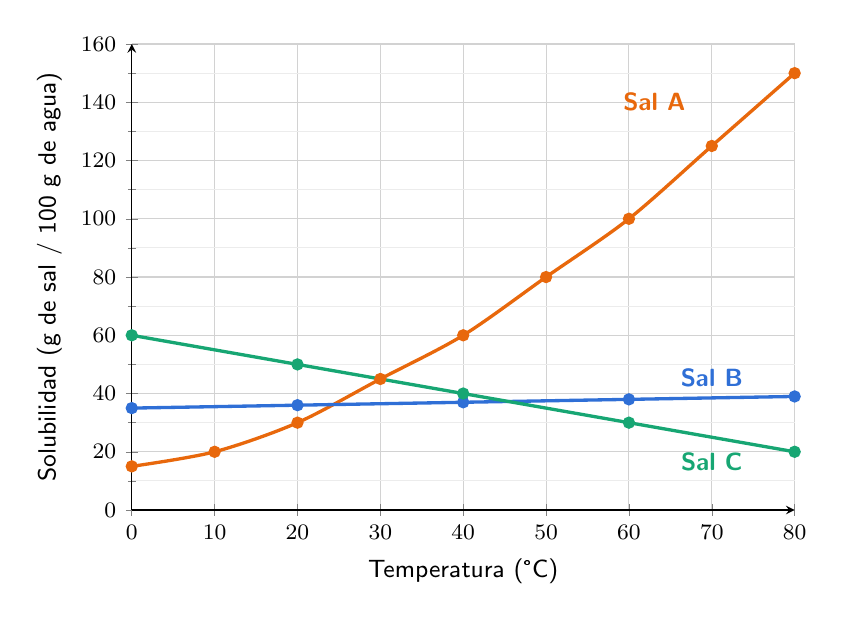
\begin{tikzpicture}[font=\small]
\begin{axis}[width=10cm,height=7.5cm,xmin=0,xmax=80,ymin=0,ymax=160,
  xtick={0,10,...,80},ytick={0,20,...,160},minor ytick={10,30,...,150},
  grid=both,major grid style={gray!35},minor grid style={gray!15},axis lines=left,
  xlabel={Temperatura (°C)},ylabel={Solubilidad (g de sal / 100 g de agua)},
  ylabel style={font=\small},xlabel style={font=\small},tick label style={font=\footnotesize}]
\addplot[nar,very thick,smooth,mark=*,mark size=1.6pt] coordinates {(0,15)(10,20)(20,30)(30,45)(40,60)(50,80)(60,100)(70,125)(80,150)};
\addplot[azul,very thick,smooth,mark=*,mark size=1.6pt] coordinates {(0,35)(20,36)(40,37)(60,38)(80,39)};
\addplot[menta,very thick,smooth,mark=*,mark size=1.6pt] coordinates {(0,60)(20,50)(40,40)(60,30)(80,20)};
\node[nar,font=\small\bfseries,anchor=east] at (axis cs:68,140) {Sal A};
\node[azul,font=\small\bfseries,anchor=south] at (axis cs:70,39) {Sal B};
\node[menta,font=\small\bfseries,anchor=north] at (axis cs:70,23) {Sal C};
\end{axis}
\end{tikzpicture}
\end{document}
